\documentclass[12pt]{article}
\usepackage{graphicx}
\usepackage{caption}
\usepackage[sort&compress]{natbib}
\usepackage{authblk}
\usepackage[utf8]{inputenc}
\usepackage{setspace}
\usepackage{rotating}
\usepackage[british]{datetime2}

\renewcommand\Affilfont{\itshape\small}

\title{Midway Evaluation Prospectus (updated)}
\author[1]{Marius Swane Wishman}
\affil[1]{Department of Sociology and Political Science, NTNU}
\date{\today}

\providecommand{\keywords}[1]
{
	\small	
	\textbf{\textit{Keywords---}} #1
}

\begin{document}

\maketitle

% \begin{abstract}

% \end{abstract}

\keywords{Artificial states, contentious politics, civil conflict, historical 
	states, state entities, state formation, civil war, ethnic conflict, 
	pre-colonial states, long history}

\pagebreak

\pagebreak

\onehalfspacing

\section{Introduction}
%The overarching research question and themes of the dissertation.

Based on the first article of the thesis, research interests, plans for 
articles 2-4 and the ARC and Geo-ISD projects, I pose the following overarching 
research question for my thesis: How do historical and pre-colonial states 
affect current contentious politics?

States have been some of the largest and most powerful organizations in the 
world ever since they fist appeared \citep{Tilly1990}.
Nevertheless, surprisingly little research has gone into what happens to states 
after they disappear from the international system of states, and what happens 
to states incorporating the such historical states.
In the first article of this thesis we show multiple examples of states 
surviving on a sub-state (no longer sovereign) level, even decades after 
disappearing from the international system of sovereign states.
Other states are dismantled by conquering states, yet live on in identities and 
histories of the inhabitants of the bygone state.
This thesis will add to a growing literature exploring long histories, how 
differences in the past experiences affects recent or current outcomes, by 
examining the long history of statehood and its effect on contentious politics 
(both violent and non-violent).

\section{Beyond Ethnicity: Dead States and Modern Conflict}

This paper started from the overarching research question: How do historical
state entities (states that are more or less `dead') affect post World War 2
levels of conflict?

The emerging/existing literature on the subject of pre-colonial and historical
(no longer sovereign states has reached differing conclusions.
Some scholars find that ethnic groups with more centralized pre-colonial
institutions experience less conflict with the central government \citep{
Wig2016} and that regions with longer histories of statehood are more peaceful
\citep{Depetris-Chauvin2016}. However, others have found that the 
conflicts of prior states can leave legacies of ethnic tension \citep{
Besley2014}.
In a recent article \citet{Paine2019} found that ethnic groups who lack a
history of statehood/centralized ethnic institutions, and find themselves 
within a country that has a group with such history, are more conflict prone 
than ethnic groups living in countries where no groups has such histories.
\citet{Paine2019} argues that this is because ethnic groups with a history of 
statehood or centralized ethnic institutions were more likely to inherit the 
state apparatus after decolonization. 
These groups would then more effectively (\emph{ceteris paribus}) exclude other 
groups from political power, leaving the excluded groups few channels to 
political power other than violence.
He also finds that in those instances where the group prior state history did 
not inherit 'the keys to the kingdom' they would also be more likely to engage
in violence to achieve political power.

% Alesina/Easterly ?

%Drawbacks: 
%* Start from the base of ethnic groups.
%* Most rely on a limited African sample.
%* Most rely on incomplete data.

Our paper makes three main contributions to the literature.
First, we do not assume that prior statehood necessarily affects conflict through
ethnic groups. 
Not all pre-colonial states were ethnic states in any meaningful sense, while
other were multi-ethnic in nature.
Some were even the foundations of current ethnic identities (the paper gives 
multiple examples).
Second, we employ new data that improves upon previous sources on pre-colonial
statehood by identifying far more states than without compromising the pre-
requisites for statehood and by having global coverage. 
Most of the literature has relied on either the \citet{Murdock1967} map of 
ethnic groups in Africa, the state antiquity data (which is global but covers 
relatively few states) or other incomplete data.
Third, we propose/construct a new measure of 'artificial statehood' that is
more in line with theory than existing measures such as the straightness of 
boundaries \citep{Alesina2011} or the variance in pre-colonial ethnic 
centralization \citep{Englebert2002}.
We measure 'artificial statehood' -- the degree to which a state overlaps with
the pre-existing topology of statehood -- as the number of historical state 
entities within its current boundaries.
We propose 4 mechanisms through which more historical state entities (HSEs)
increase the chance of civil conflict: HSEs (1) created networks useful for 
insurgency, (2) were symbols of past sovereignty, (3) generated modern ethnic
groups that activated dynamics of ethnic inclusion and exclusion and (4)
resisted western colonialism and specific values it brought with it.

Our hypothesis is:

\bigskip
\textit{H\textsubscript{1}: More historical states in the territory of a state
increases the number of internal armed conflicts.}
\bigskip

We find a robust positive association between more HSEs inside a modern state 
and the number of civil conflict onsets between 1946-2019. 
This relationship is not driven by common explanations of state-formation that 
also drive conflict such as the number of ethnic groups, population density, 
colonialism, levels of historical warfare, or other region specific factors.
Using mediation analysis we find some moderate support for the colonialism 
mechanism, although a strong independent effect of more historical state 
entities on civil conflict onsets remains across all models. 

\bigskip
Status: Awaiting response from JPR.

\section{Geo-ISD Project}

Together with Charles Butcher and research assistant Eirin Haugseth the project
aimed to create geocoded information for the African historical state entities
in the original ISD data set.  Specifically, on the locations and borders of
these historical state entities. The resulting data provides a far clearer view
of not just how many pre-colonial states there were in Africa, but also where
these were and -- so we argue -- over what areas they had more or less control.

The data has been collected, compiled and cleaned (mostly), and has been
integrated not just with the original ISD, but with the PRIO-GRID system of
geo-data as well.

The resulting papers using this data (covered in the subsections below) will
form the bulk of my thesis.

\subsection{The data}

To get the locations of different historical state entities we used a
combination of maps from the time period covered by the ISD and maps found in
historical atlases compiled by historians in our own time.  The historically
contemporary maps were collected from the David Rumsey project at
davidrumsey.com.  We then georeferenced the maps and traced polygons for the
states included in both the map and the ISD.  Similarly the historical atlases
were scanned, georeferenced and relevant state entities were traced.

In the end we were left with over 3400 polygons covering the period 1800 to 1914
for continental Africa and Madagascar. For some HSE's in the ISD we have no maps
for any years, some are covered only for some of the years they are in the ISD,
but a substantial number of them are covered by multiple maps for many years.
%TODO Find exact percentages.
% TODO Check how many unique states from the ISD is included in the Geo-ISD.
When maps disagreed on where the various borders were in a given year, we take
it as an indication of the ambiguity of where a given state had \emph{de facto}
or \emph{de jure} control in that year. In some areas all the maps would overlap
(at the very least in the immediate surroundings of the capital), while in other
areas they would not. In the areas where all the maps agree we could be quite
sure that the given state entity had real presence. While in areas where only
one map indicated that the state was presence, this could either be wrong, an
indication of \emph{de jure} as opposed to \emph{de facto} presence or some
other form of limited presence. The coding process of looking at hundred of maps
strengthened this initial intuition, and the resulting figures of state presence
drawn from the complete data lends it further credence. 

The data from this project can be aggregated and used in many ways and to
produce many variables. Initially, I have opted on 14 slightly different
measures of state presence, 3 of which are considered the main measures of three
unique aspects of state presence, the rest are more or less conservative
versions of these three. All of these indicators are aggregated over all years
for individual PRIO-GRID cells in Africa. The first indicator is a measure of
the presence of one state over time \ref{sp}. It is measured by the number of
maps that indicate that a state was present there, counting only those of the
state most often present in that cell. The second is a measure of overlapping
sovereignty and is the number of times that two or more maps in a year disagrees
on which state was present in that grid cell, summed over all years \ref{sp_o}.
The third is a measure of the degree to which a grid cell was a frontier-, or
border region \ref{sp_b}. It counts the number of maps that indicate that a
border ran through the grid cell.

\begin{figure}[!htb]
	\caption{State presence}
	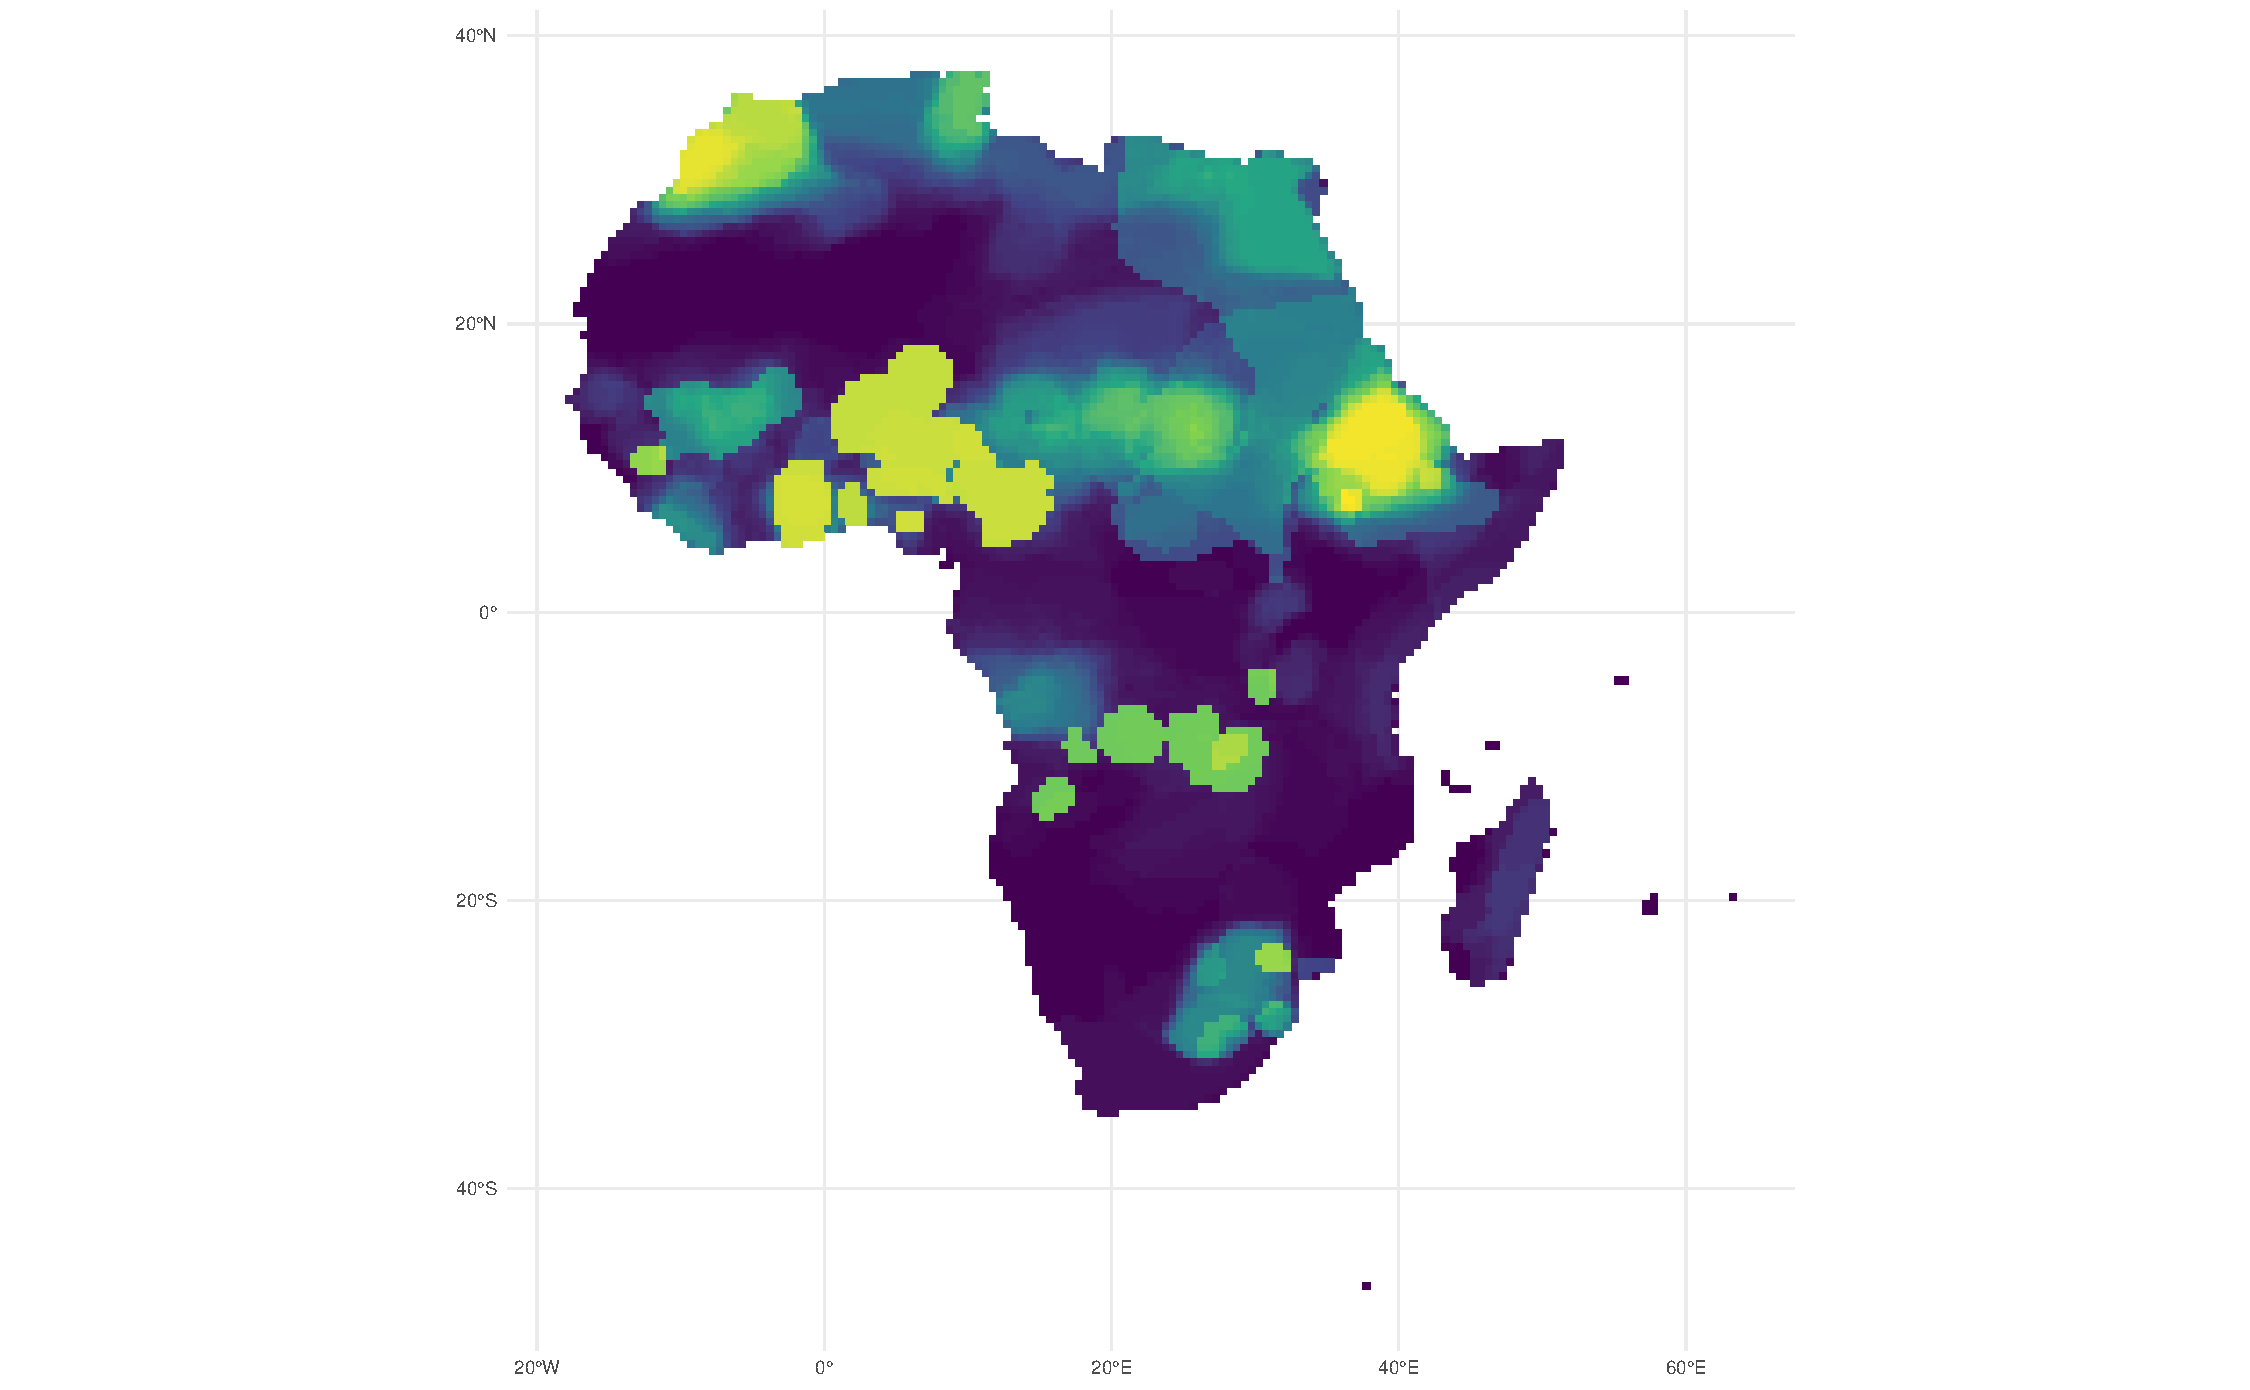
\includegraphics[width=\textwidth,keepaspectratio]{sp_sum_i_any.pdf}
	\label{sp}
\end{figure}

\begin{figure}[!htb]
	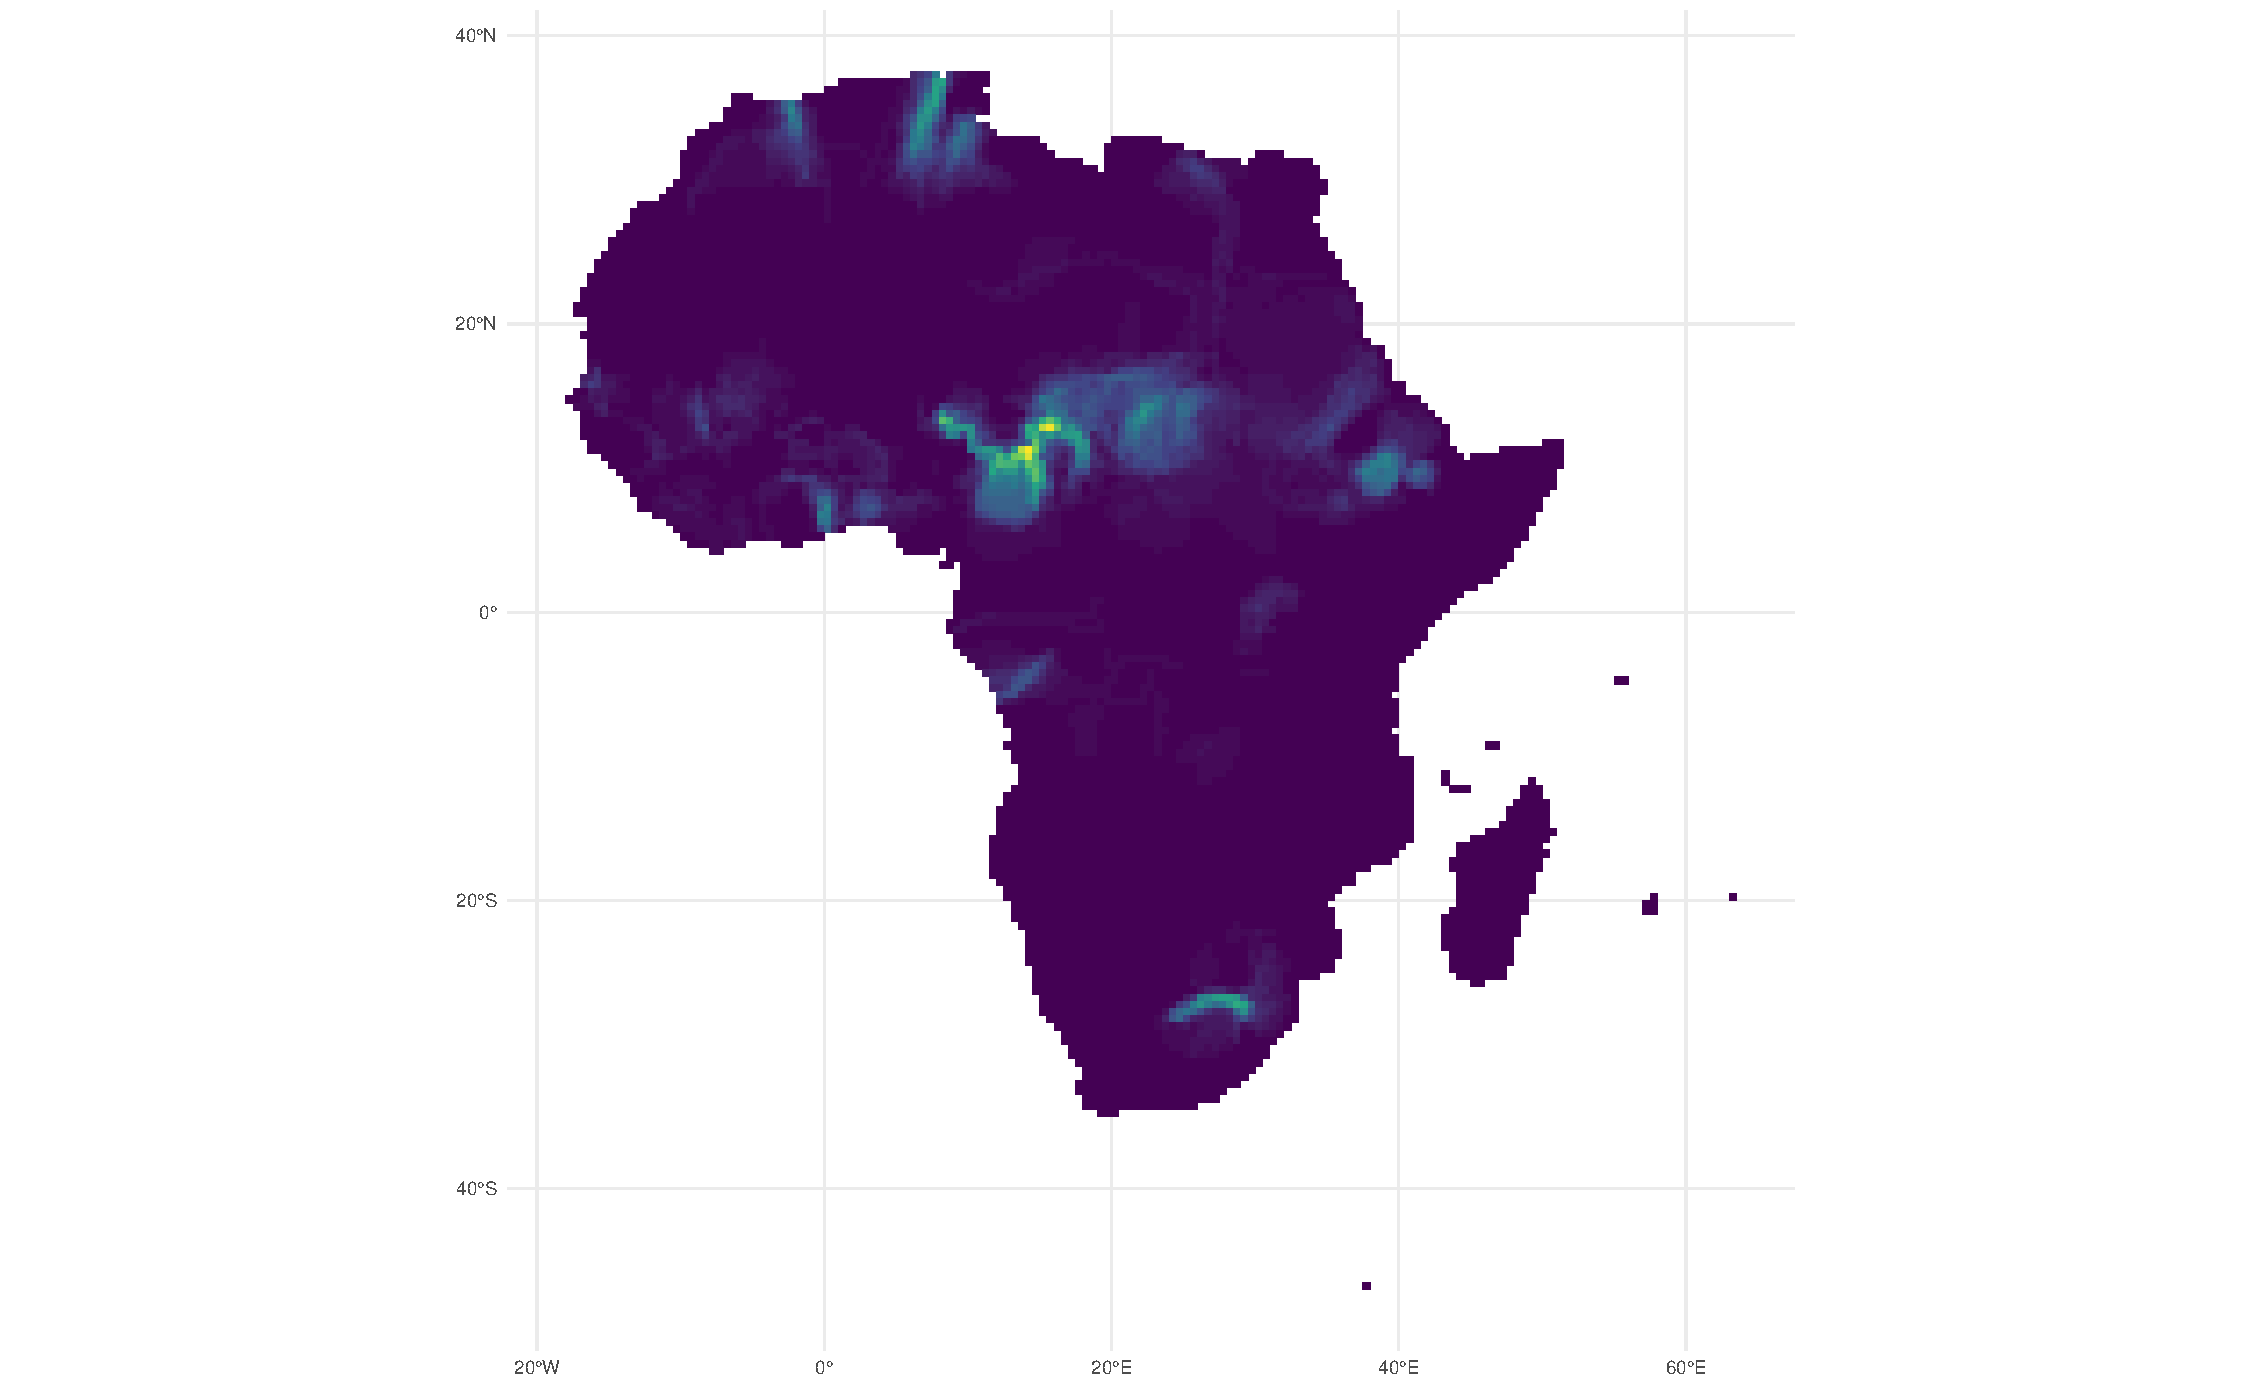
\includegraphics[width=\textwidth,keepaspectratio]{sp_o.pdf}
	\caption{Overlapping state presence}
	\label{sp_o}
\end{figure}

\begin{figure}[!htb]
	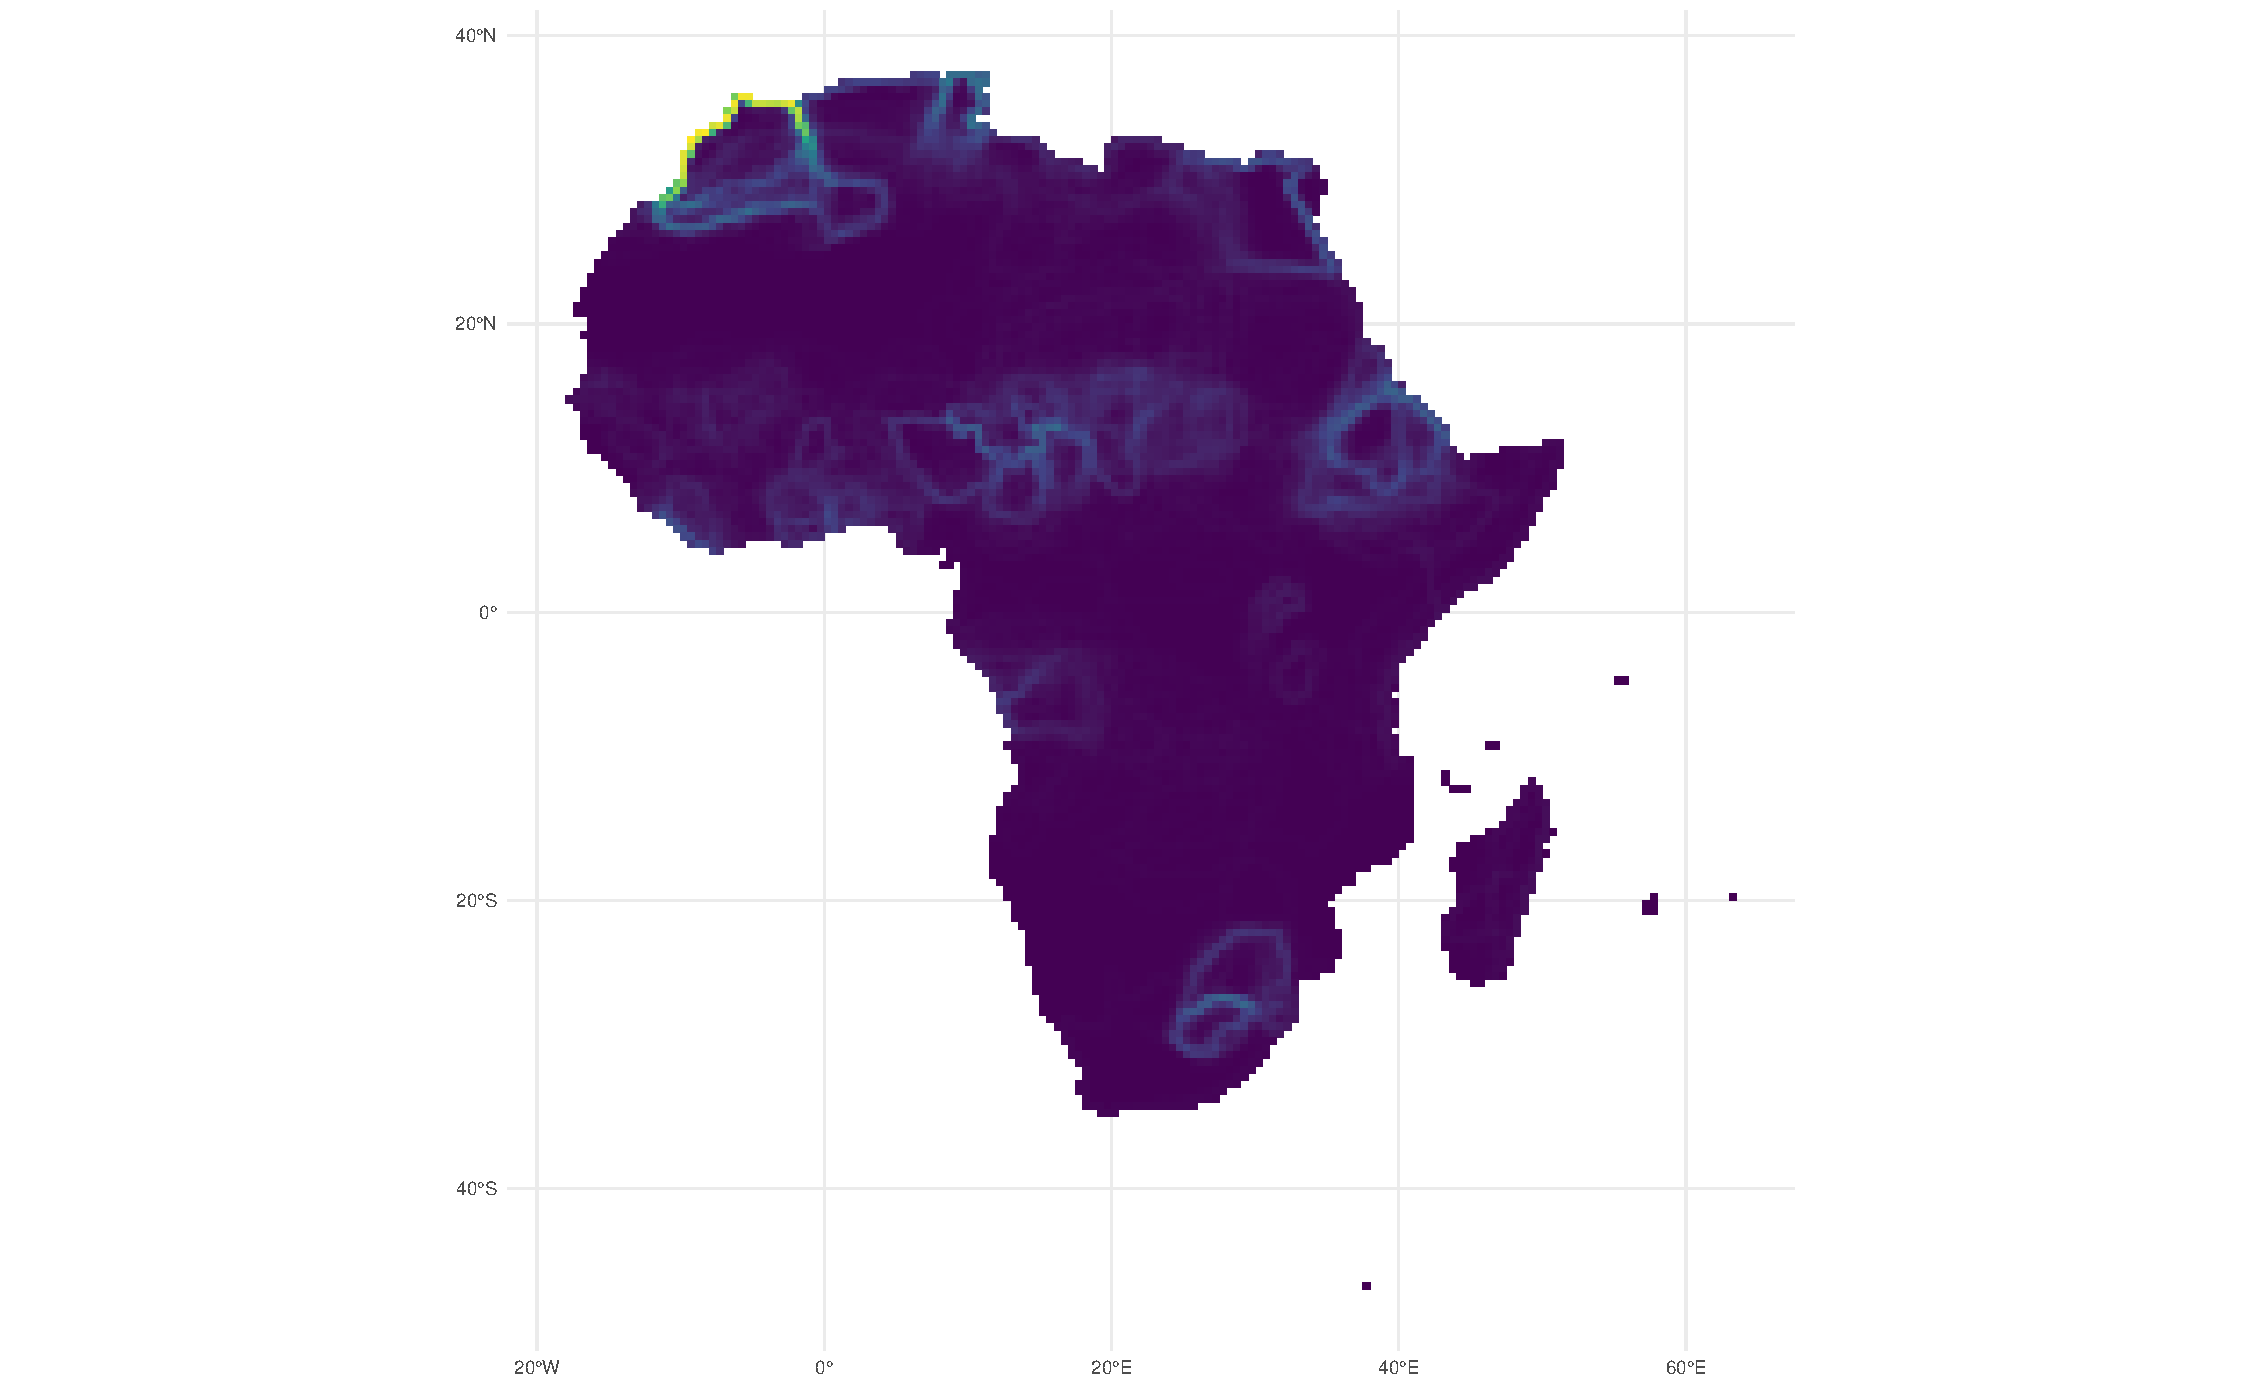
\includegraphics[width=\textwidth,keepaspectratio]{sp_b_sum.pdf}
	\caption{Borders}
	\label{sp_b}
\end{figure}

\subsection{Historical states and civil conflict}

Based on the Geo-ISD data I plan to write a paper testing some of the key
theories and assumptions surrounding state presence, pre-colonial statehood and
civil conflict.

There is a considerable literature focusing on the pacifying effect of state
presence over time leading to more peaceful societies. \citet{Bockstette2002}
argued that states through fostering a sense of nationhood and common language
can prevent civil war and political instability. In support of this view they
find that their State Antiquity Index correlates positively with several
measures of political stability. \citet{Tilly1990} argues that over time the
state monopolizes the use of violence and over time out competes any challengers
to this monopoly. \citet{Pinker2012} synthesised a lot of this literature and
shows empirically that societies tend to get less violent at every level after
the advent of states and increasingly so with the increasing penetration of the
modern state into the societies it governs.

The literature that focuses more the special case of HSE's or pre-colonial
states, and conflict has drawn more mixed conclusions. Some scholars find that
HSE's are  locally peace inducing \citep{Wig2016, Depetris-Chauvin2016}, while
others find that grid cells that had been part of historical kingdoms were more
likely to have legacies of conflict that in turn increased the likelihood of
modern conflict. At the national level as well pre-colonial statehood can lead
to conflict, by making ethnic groups with a history of statehood better able to
exclude others from power, or better equipped to violently challenge a dominant
group should they themselves be excluded \citep{Paine2019}. In the first paper
of the thesis we found a positive association between the number of HSE's and
civil conflict, and proposed some potential mechanisms through which they could
be related. The Geo-ISD will allow me to test these mechanisms further. However,
that could prove to be outside the scope of this paper.

The overall prediction of the literature at a grid cell level would be that
increased exposure to statehood, should decrease the likelihood of civil
conflict, after controlling for factors that could affect both local conditions
for state formation and conflict.

\subsection{Historical states and communal violence}

Ole Magnus Thiesen had the idea to use the Geo-ISD data to look into the
relation between HSE's and communal violence (a topic he is familiar with). The
following is a rough outline of the idea for that paper as it currently stands.

The level of violence in non-state societies is qualitatively different from
that of within states with rates of violence often being several orders
magnitude higher in the former \citep{Pinker2012}. Part of this can be explained by
that one of states’ primary objectives and defining characteristics is to solve
the security dilemma \citep{Lake_1996}. Several states
in contemporary sub-Saharan Africa are judicially effective, but empirically
less so \citep{Jackson_1982}, in particular when it comes to solving the
security dilemma. This has resulted in pockets where resolution of violent
conflicts is frequently left to local traditional conflict resolution
mechanisms, where there is no neutral arbiter to mediate or enforce peace should
things get out of hand. While most of the time being able to resolve conflicts
relatively peacefully, these institutions rely on the very real threat of deadly
violence in itself in order to be credible \citep{Fearon_1996, Eaton_2007,
Eaton_2008}. In areas where feuding has remained an accepted way of resolving
disputes between communities, large-scale inter-ethnic violence is more likely
to occur \citep{Witsenburg2012} as the state is unable to ‘contain fear’ in
an effective and unbiased manner \citep{Lake_1996}.  

There might be variations in this semi-anarchic situation, however, as some
areas have a long pre-colonial legacy of statehood which previously have
addressed the security dilemma between ethnic groups. While it is an open
question of how effective such institutions are in resolving disputes that have
escalated into violence between communities, they have proven effective in
reducing the number of less serious disputes that could escalate, thereby
reducing the overall number of disputes that could escalate. In general
therefore, where states existed prior to colonization, the risk of
inter-communal violence should be lower. Indeed, \citet{Wig2018} found that
ethnic groups that were recorded as having more centralized institutions by the
\citet{Murdock1967} were less likely to experience communal violence.

Pre-colonial state-structures can reduce conflict potential in at least three
partly separate ways. First, in some instances these institutions are present in
themselves to a greater or lesser extent in modern states, but operate outside
formal state structures. This could represent an efficient way of resolving
low-level disputes that have escalatory potential.  Case studies from South
Saharan Africa indicate that if a resource dispute arises…locals prefer to turn
first to friends, neighbours and relatives, before resorting to traditional
authorities like village elders or a chief \citep{Turner_2012}.  Formal
institutions are at this stage often shunned. They are seen as less in touch
with the local context, thus making inflexible judgements; being more costly and
corrupt; and creating long-standing grievances between families.  The presence
of pre-colonial institutions today can therefore represent a more trusted venue
for resolving disputes, in turn reducing the pool of incidences with escalatory
potential.  

Second, and partly in contrast to the above hypothesis, in some settings,
pre-colonial institutions have been formally integrated into the state, the
prime example being the integration of chiefs and kingdoms in contemporary
Ghana. Studies using Afrobarometer data show that trust in traditional
institutions translates into trust in modern institutions \citep{Logan_2009}.
This relation arguably also goes the other way, as informal institutions are
more fragile if not recognized by the state \citep{ostrom1990governing}. As
there is some notion of British rule effectively being more indirect (thus not
only in name) than former French and Lusophone colonies and therefore in the
former pre-colonial states have been more effectively been incorporated in
colonial and post-colonial states. 

Third, pre-colonial states have left an imprint in terms of norms of intergroup
behaviour that is different from areas without a legacy of pre-colonial
statehood. By having reduced the security dilemma in past times, pre-colonial
states have often facilitated the co-habitation of different ethnic groups in
the same settlements, hence reducing the kind of segmentation often found in
feuding societies (see e.g. Diamond 2012).

\subsection{Historical states and non-violent resistance}

An idea for a potential third paper using the Geo-ISD (among many other ideas)
could be looking for a potential relationship between HSE's and non-violent
resistance. The benefit of following this idea for me is that it would help the
tie the PhD together as a whole, by providing a `missing link' between my
research on HSE's and the work I have done on the ARC project in general and the
data release paper in particular.

Potential mechanisms: HSE's leave networks that facilitate mobilization (for
non-violent resistance as well). Familiarity of interaction with state
institutions (however changing). Parallel much of the literature that suggests
that HSE's are locally peace inducing, as they imply that conflicts and
potential conflicts are resolved in non-violent ways, perhaps some of these are
picked up by measures of non-violent resistance. The implication would be that
areas with a `thicker' state presence would be more likely to experience
non-violent rather than violent resistance to the state.

A different avenue to approach this could be that HSE's could leave behind
non-state institutions, or foundations on which modern institutions could be
built. The testable implication of this would be that grid cells with 'thicker'
state presence would be more likely to see activity be more highly organized
organisations such as trade unions or political parities.

As you can tell, not much though has gone into this last paper yet. Luckily, the
data I have now has opened a lot of opportunities for potential papers. By the
time I have finished the papers that I have started on, I will probably have a
clear idea of exactly what I want to do for the last paper.

\section{ARC data release paper}

Finally, I will also co-author the data release paper from the Anatomy of 
Resistance Campaigns (ARC) project.
The paper introduces the ARC data set on groups participating in violent an non-
violent maximalist dissent in Africa over the period 1990-2015.

% \section{Other Ideas}

% %How Wilson changed the interaction between ethnicity and statehood.

% Building on the second paper.
%Many African democracies struggle with fractious party systems, with large 
%numbers of regional and ethnic parties competing to capture spoils of the state 
%(jobs, aid-programs, financial transfers, development projects etc.).
%Through similar mechanisms as described in the second paper expect more cohesive 
%countries to be better able to form policy-based political parties that span 
%regions and ethnic groups.
%\bigskip

\section{Progress}

In terms of the articles that will form part of the thesis, the first one was
rejected by International Organization. We tried to implement some of the
feedback from reviewers as well as our collogues, and have now submitted the
paper to JPR where we are awaiting a response.  

The next step is finishing the last little bits of clean-up on the Geo-ISD, and
of course write the remaining articles,beginning with the ones on HSE's and
civil conflict and communal violence. I have also begun writing an article of
sorts on the Geo-ISD, about the process, motivation and so on. Similarly, I have
started writing a literature review on statehood and internal conflict. Both of
these are primarily intended to be used for the articles sketched out above,
but might become separate articles in their own right.

Overall I am content with the rate of progress so far, despite only having 
submitted one article for review.
This is because I believe I now have a clearer idea of what the rest of the 
thesis will look like, and how I will go about writing it.
Additionally, all of the duties to the department are done.
After this semester there will only be approximately 30 hours remaining.
I have also finished the requisite methods and philosophy of science courses 
that are part of the PhD Program.
10 ETC points worth of substantive course(s) remain.

Lastly, I plan to go on parental leave for 15 weeks from early November.

\pagebreak
\bibliographystyle{agsm}
\bibliography{lib.bib}
\end{document}
